%=============================================================================
% Traffic Digital Twin — IEEE conference report (WITH Contribution section)
% Identical to report_base.tex plus Section "Contribution" before References.
% Compile: pdflatex report_contribution ; bibtex report_contribution ; pdflatex x2
% Or upload the report/ folder to Overleaf and compile report_contribution.tex.
%=============================================================================
\documentclass[conference]{IEEEtran}
\IEEEoverridecommandlockouts

\usepackage{cite}
\usepackage{amsmath,amssymb,amsfonts}
\usepackage{algorithm}
\usepackage{algpseudocode}
\usepackage{graphicx}
\usepackage{booktabs}
\usepackage{textcomp}
\usepackage{xcolor}
\usepackage{tikz}
\usetikzlibrary{shapes.geometric, arrows.meta, positioning, fit, backgrounds}
\usepackage[hidelinks]{hyperref}
\usepackage{url}
\usepackage[final]{microtype}

% Long monospaced identifiers (e.g. transform.py:\_pixel\_to\_gps\_curved) cannot
% break in the narrow IEEE columns and cause large inter-word gaps. Allow a break
% after every underscore and relax justification slightly to remove the rivers.
\renewcommand{\_}{\textunderscore\allowbreak}
\setlength{\emergencystretch}{3em}

\graphicspath{{img/}{figures/}{../poster/}}

% Compile-safe figure: include the image if present (searched in figures/ and
% ../poster/ via \graphicspath), else draw a labelled placeholder. \detokenize keeps
% underscores in filenames from being read as math.
\newcommand{\figorbox}[2]{%
  \IfFileExists{img/#1}{\includegraphics[width=\linewidth]{#1}}{%
  \IfFileExists{figures/#1}{\includegraphics[width=\linewidth]{#1}}{%
  \IfFileExists{../poster/#1}{\includegraphics[width=\linewidth]{#1}}{%
  \IfFileExists{#1}{\includegraphics[width=\linewidth]{#1}}{%
    \fbox{\parbox[c][3.2cm][c]{0.92\linewidth}{\centering\small\itshape
      [figure placeholder: \texttt{\detokenize{#1}}]\\#2}}}}}}}

\begin{document}

\title{A Real-Time Traffic Digital Twin from Public CCTV:\\
Vision-Based Detection, Map-Anchored Localization, and Self-Calibrating Speed Estimation}

\author{
\IEEEauthorblockN{Minsoo Ahn}
\IEEEauthorblockA{Department of Computer Science\\
Stony Brook University\\
minsoo.ahn@stonybrook.edu}
\and
\IEEEauthorblockN{Dahyun Kwon}
\IEEEauthorblockA{Department of Computer Science\\
Stony Brook University\\
dahyun.kwon@stonybrook.edu}
}

\maketitle

%-----------------------------------------------------------------------------
\begin{abstract}
We present a real-time traffic digital twin that converts live public CCTV feeds
into an interactive, map-anchored view of road traffic. From a single clicked
camera the system streams HLS video, detects vehicles with YOLOv8 and tracks them
with a pluggable multi-object tracker (BoxMOT), and converts each vehicle's pixel
position to a geographic coordinate through a perspective homography. Because
public CCTV cameras are uncalibrated and their intrinsics are unknown, accurate
ground-plane mapping and speed estimation are the central challenges. We address
them with three complementary mechanisms: (i) a two-stage \emph{curved} transform
that maps pixels along the true road centreline obtained from the national
node-link road network rather than a flat plane; (ii) a five-stage speed estimator
combining a physics-based outlier guard, least-squares regression over a sliding
window, and per-track exponential smoothing; and (iii) an online self-calibration
loop that compares the measured speed against the official ITS segment speed and
learns a per-camera correction factor. The system additionally provides
multi-camera background monitoring, camera-level congestion clustering, and a
SQLite time-series history with charting. We describe the architecture and the key
algorithms, and report latency, throughput, tracking-stability, and speed metrics
produced by a measurement harness over live streams.
\end{abstract}

\begin{IEEEkeywords}
digital twin, intelligent transportation systems, object detection, multi-object
tracking, homography, perspective transform, speed estimation, real-time
visualization.
\end{IEEEkeywords}

%=============================================================================
\section{Introduction}
%=============================================================================
Cities expose thousands of public traffic cameras, but the raw feeds are difficult
to interpret at scale: an operator watching a video grid cannot read off vehicle
counts, speeds, or where congestion is forming on a map. A \emph{digital twin}---a
live, geo-referenced model of the road state---turns those feeds into actionable
information. The technical obstacle is that public CCTV cameras are
\emph{uncalibrated}: their height, pitch, focal length, and exact heading are
unknown, so projecting an image detection onto the ground plane (and therefore
measuring distance and speed) is ill-posed without per-camera calibration.

This paper describes a system that ingests Korean ITS CCTV streams and produces a
real-time map-anchored twin. Our contributions, from a systems and algorithms
standpoint, are:

\begin{itemize}
  \item \textbf{Map-anchored localization.} We snap each camera onto the national
  node-link road network, extract the road centreline, and map pixels along the
  \emph{curve} of the road in two stages, rather than assuming a flat homographic
  plane. This keeps vehicle markers on the road even on bends.
  \item \textbf{Robust speed estimation without ground truth.} A five-stage filter
  (duplicate skip, physics jump guard, sliding-window least-squares regression,
  per-track exponential smoothing with spike rejection, and scale correction)
  produces stable speeds despite detection jitter and tracker ID churn.
  \item \textbf{Online self-calibration.} Because absolute scale is unknowable from
  an uncalibrated camera, we learn a per-camera \texttt{speed\_scale} by comparing
  our measured average against the ITS official segment speed, with convergence and
  volatility guards.
  \item \textbf{A complete, resilient pipeline.} Automatic lane-based calibration,
  manual 4-point calibration, dual-path inference (browser canvas and server-side
  HLS) over a shared detector, multi-camera background monitoring, congestion
  clustering, and a historical analytics store.
\end{itemize}

The rest of the paper is organized as follows. Section~\ref{sec:related} reviews
related work. Section~\ref{sec:design} presents the system architecture.
Section~\ref{sec:impl} details the algorithms. Section~\ref{sec:eval} reports the
measurements. Section~\ref{sec:discuss} discusses limitations, and
Section~\ref{sec:concl} concludes.

%=============================================================================
\section{Related Work}\label{sec:related}
%=============================================================================
\textbf{Object detection and tracking.} Modern traffic vision builds on real-time
detectors; we use YOLOv8~\cite{yolov8} for its speed/accuracy balance and TensorRT
FP16 execution~\cite{tensorrt}. For tracking we use the BoxMOT
framework~\cite{boxmot}, which exposes ByteTrack~\cite{bytetrack},
BoT-SORT~\cite{botsort}, and OC-SORT~\cite{ocsort}; appearance re-identification
uses OSNet~\cite{osnet}. Trackers without appearance ReID suffer ID switches under
occlusion, which we mitigate with a lightweight position-based ID stabilizer.

\textbf{Camera-to-ground mapping.} Mapping image points to a ground plane is a
homography problem~\cite{hartley2004}, typically solved from four correspondences
with OpenCV~\cite{opencv}. For \emph{uncalibrated} cameras, vanishing-point and
lane-geometry cues are commonly used to recover pose. Our work combines a
4-point manual mode, a vanishing-point/lane auto-calibration, and---novel in this
context---a road-centreline-following transform driven by an external road-network
dataset~\cite{moct_nodelink}.

\textbf{ITS dashboards and data.} National ITS portals~\cite{its_openapi} publish
CCTV streams and aggregated segment speeds, but typically as separate views. We
\emph{fuse} the segment speed back into the pipeline as a calibration signal.
Congestion grouping uses density-based clustering~\cite{dbscan} and convex
hulls~\cite{andrew1979}; service levels follow the Highway Capacity
Manual~\cite{los_hcm}. The visualization uses deck.gl~\cite{deckgl} over
MapLibre~\cite{maplibre}, served by FastAPI~\cite{fastapi}.

%=============================================================================
\section{System Design and Architecture}\label{sec:design}
%=============================================================================
The backend (FastAPI/Uvicorn) and a React/deck.gl frontend communicate over REST
and WebSocket. Two inference paths can produce per-frame analytics and
\emph{share a single detector}; a connection counter coordinates them so that the
multi-object tracker is never driven by two interleaved frame streams.

\begin{figure}[t]
\centering
% --- Architecture diagram (TikZ; self-contained, no external image needed) ---
\resizebox{\linewidth}{!}{%
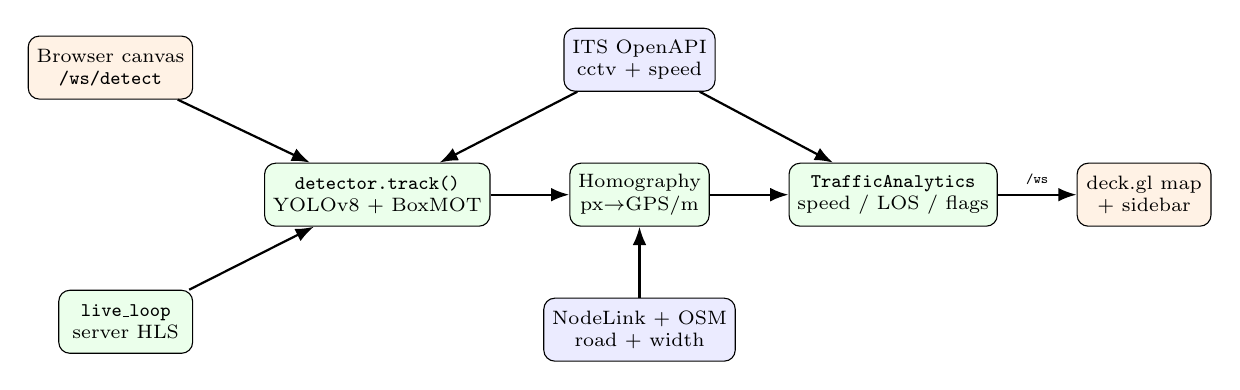
\begin{tikzpicture}[
  box/.style={draw, rounded corners, align=center, font=\scriptsize, inner sep=3pt,
              minimum height=8mm, minimum width=17mm},
  ext/.style={box, fill=blue!8},
  be/.style={box, fill=green!8},
  fe/.style={box, fill=orange!10},
  arr/.style={-{Latex}, thick}]

  % main pipeline (single row, left to right)
  \node[be] (det) {\texttt{detector.track()}\\YOLOv8 + BoxMOT};
  \node[be, right=10mm of det] (tf) {Homography\\px$\to$GPS/m};
  \node[be, right=10mm of tf] (an) {\texttt{TrafficAnalytics}\\speed / LOS / flags};
  \node[fe, right=10mm of an] (ws) {deck.gl map\\+ sidebar};

  % two inputs merge into the shared detector (left side)
  \node[fe, above left=8mm and 9mm of det] (canv) {Browser canvas\\\texttt{/ws/detect}};
  \node[be, below left=8mm and 9mm of det] (live) {\texttt{live\_loop}\\server HLS};

  % external data sources (above / below the centre, short non-crossing arrows)
  \node[ext, above=9mm of tf] (its) {ITS OpenAPI\\cctv + speed};
  \node[ext, below=9mm of tf] (nl)  {NodeLink + OSM\\road + width};

  \draw[arr] (canv) -- (det);
  \draw[arr] (live) -- (det);
  \draw[arr] (det)  -- (tf);
  \draw[arr] (tf)   -- (an);
  \draw[arr] (an)   -- node[above,font=\tiny]{\texttt{/ws}} (ws);
  \draw[arr] (nl)   -- (tf);
  \draw[arr] (its)  -- (det);
  \draw[arr] (its)  -- (an);
\end{tikzpicture}}
\caption{System architecture. The browser path (\texttt{/ws/detect}) and the
server path (\texttt{live\_loop}) share one detector; a counter prevents concurrent
tracker calls. External data (ITS CCTV/speed, NodeLink, OSM) feeds localization and
self-calibration.}
\label{fig:arch}
\end{figure}

\textbf{Browser path (\texttt{/ws/detect}).} The frontend plays the HLS stream
through a CORS proxy, captures canvas frames (JPEG, $\le$640\,px, $\approx$33\,ms
interval, at most two in flight), and sends them to the backend, which runs
detection, tracking, localization, and analytics, then returns an annotated frame
and broadcasts the analytics JSON to all clients.

\textbf{Server path (\texttt{live\_loop}).} The backend can also read the HLS
stream directly with OpenCV/FFmpeg and run the same pipeline. It is gated twice: it
skips tracking while a browser detection client is active (to protect the shared
tracker), and it skips all GPU work when no one is watching (the frontend reports
tab visibility).

\textbf{Background services.} Periodic loops refresh expiring HLS tokens (30\,min),
poll the ITS segment speed for self-calibration (5\,min), and snapshot all monitored
cameras into a SQLite history while recomputing congestion clusters (30\,s). The
resulting map view is shown in Fig.~\ref{fig:map}.

\begin{figure}[t]
\centering
\figorbox{cctv_map.png}{Map view with status-coloured CCTV icons and FOV polygon}
\caption{Map view: public CCTV cameras as status-coloured icons on the vector map;
the selected camera shows its field-of-view polygon and the located vehicles.}
\label{fig:map}
\end{figure}

%=============================================================================
\section{Implementation}\label{sec:impl}
%=============================================================================

\subsection{Detection and Tracking}
The detector loads the fastest available backend---TensorRT FP16 engine, then ONNX
Runtime, then PyTorch---and exports \texttt{.pt}$\to$\texttt{.engine} on first run
when a GPU is present. A tracker \emph{tier} is chosen by GPU memory: ByteTrack
(CPU/low-VRAM), OC-SORT (occlusion-robust, no ReID), or BoT-SORT/DeepOC-SORT with
OSNet appearance ReID on larger GPUs. For the non-ReID tiers we add two robustness
layers: \texttt{\_dedup\_tracks} merges duplicate boxes (IoU\,$>$\,0.3 or centre
distance\,$<$\,40\,px, keeping the older ID), and an \texttt{IDStabilizer}
re-binds a vehicle's previous ID after a brief miss using nearest-centre matching
($\le$80\,px) with a two-pass scheme and stale-mapping purge so display IDs stay
stable and compact. Fig.~\ref{fig:yolo} shows the detection and tracking overlay.

\begin{figure}[t]
\centering
\figorbox{yolo_detect.png}{YOLO detection and multi-object tracking overlay}
\caption{Detection and tracking on a live CCTV frame: bounding boxes, vehicle class,
and stabilized track IDs.}
\label{fig:yolo}
\end{figure}

\subsection{Map-Anchored Localization}
On camera switch we query the national node-link network: we snap the camera
position perpendicularly onto the nearest road polyline, extract $\pm$150\,m of
centreline, and---because each direction is stored as a separate one-way link---we
locate the reverse carriageway and average the two snaps (when 2--40\,m apart) to
recover the true road centre. The chosen road's speed limit, lane count, and width
(\,lanes\,$\times$\,2\,$\times$\,lane-width\,) are attached to the camera; OSM
Overpass provides a width refinement when available.

Given the centreline, the \emph{two-stage curved transform} maps a pixel
$(u,v)$ to GPS along the road (Algorithm~\ref{alg:curved}): stage one maps the pixel
to local metres via the metric homography; stage two decomposes the displacement
from the snap point into along-road and lateral components, advances that arc length
along the centreline, interpolates the on-road position, and re-applies the lateral
offset perpendicular to the \emph{local} road bearing. This follows real road
curvature, unlike a single flat homography.

\begin{algorithm}[t]
\caption{Two-stage curved pixel$\to$GPS transform}
\label{alg:curved}
\begin{algorithmic}[1]
\Require pixel $(u,v)$; metric homography $H_m$; centreline \textit{road\_pts};
         \textit{snap\_along}; direction sign $s$
\State $(x_m,y_m) \gets H_m \cdot (u,v)$
\State $(dx,dy) \gets (x_m,y_m) - \textit{snap}_m$ \Comment{ENU from snap}
\State $d_{\parallel} \gets dx\sin b + dy\cos b;\quad d_{\perp} \gets dx\cos b - dy\sin b$
\State $\textit{arc} \gets \textit{snap\_along} + s\cdot \max(0,d_{\parallel})$
\State $(\textit{lat},\textit{lon}) \gets \textsc{InterpCenterline}(\textit{arc})$
\State $b_\ell \gets \textsc{RoadBearingAt}(\textit{arc})$
\State \textbf{apply} $d_{\perp}$ perpendicular to $b_\ell$ \Return $(\textit{lat},\textit{lon})$
\end{algorithmic}
\end{algorithm}

When no manual calibration exists, an automatic procedure estimates a homography
from one frame: Canny edges in the lower image, Hough line filtering, multi-row
sampling of left/right road edges, least-squares edge fits, vanishing-point
intersection, a pitch/height estimate from a pinhole model, and a trapezoid-to-GPS
homography. Direction (which way the camera looks along the road) is resolved by
matching the \emph{image} road-curve sign against the \emph{map} curve sign, falling
back to a vanishing-point heading test. A manual 4-point mode remains available for
maximum accuracy. Fig.~\ref{fig:calib} shows an automatic calibration result.

\begin{figure}[t]
\centering
\figorbox{auto_calib.png}{Automatic lane-based calibration result}
\caption{Automatic calibration: detected lane edges and the estimated vanishing point
yield the ground homography and the field-of-view footprint.}
\label{fig:calib}
\end{figure}

\subsection{Speed Estimation}
Speed is distance over time, and both terms are error-prone: homography distance is
noisy at the far field, and HLS buffering makes naive frame timing wrong. We use a
monotonic clock derived from stream presentation timestamps (falling back to
wall-clock), and the five-stage estimator of Algorithm~\ref{alg:speed} with the
constants in Table~\ref{tab:const}.

\begin{algorithm}[t]
\caption{Per-track speed estimation (\texttt{analytics.\_speed})}
\label{alg:speed}
\begin{algorithmic}[1]
\State \textbf{(1)} skip duplicate metric positions (non-detection frames)
\State \textbf{(2)} \textbf{if} $\textit{step} > (\tfrac{V_{\max}}{3.6\,\sigma})\,dt\cdot 1.5$ \textbf{then} drop sample, keep window
\State \hphantom{(2)} \textbf{if} $dt>2$s \textbf{then} clear window
\State \textbf{(3)} fit velocity by least squares over the $W{=}18$-frame window;
\State \hphantom{(3)} \textbf{if} window displacement $<0.5$m \textbf{then} $v\gets 0$
\State \textbf{(4)} EMA: $v_e \gets (1-\alpha)v_e + \alpha (v\sigma)$, $\alpha{=}0.35$;
\State \hphantom{(4)} reject spike if $v_e{>}5 \wedge v\sigma{>}2.5v_e{+}20$; decay when stopped
\State \textbf{(5)} output $v_e$; \textbf{is\_speeding} $\gets v_e > \textit{limit}$
\end{algorithmic}
\end{algorithm}

\begin{table}[t]
\caption{Key speed/analytics constants (\texttt{config.py}).}
\label{tab:const}
\centering
\footnotesize
\begin{tabular}{@{}ll@{}}
\toprule
Parameter & Value \\
\midrule
Speed window $W$ & 18 frames \\
EMA $\alpha$ & 0.35 \\
Jitter threshold & 0.5 m \\
Min speed (else 0) & 5 km/h \\
Max plausible $V_{\max}$ & 180 km/h \\
GC grace & 30 frames \\
Bottleneck dwell & 150 frames ($\approx$5 s) \\
Parked dwell & 300 frames ($\approx$10 s) \\
LOS thresholds A--E & $\le$3,6,9,12,15 (else F) \\
\bottomrule
\end{tabular}
\end{table}

\subsection{Online Self-Calibration}
The absolute distance scale of an uncalibrated camera is unknowable, so a residual
scale error persists after geometric calibration. Every five minutes we fetch the
ITS official segment speed near the camera and update a per-camera factor
\texttt{speed\_scale}:
\begin{equation}
\textit{target} = \textit{scale}\cdot \frac{v_\text{ITS}}{\bar v_\text{ours}},\quad
\textit{scale} \gets (1{-}\alpha)\,\textit{scale} + \alpha\,\textit{target},
\end{equation}
clamped to $[0.3,5.0]$, using a 10-minute rolling average ($\ge$50 samples), a
coefficient-of-variation guard ($\le$0.4) to skip volatile traffic, and a learning
rate that drops from $0.5$ to $0.95$ once converged (three consecutive $<$1\,\%
updates). The converged factor is persisted per camera.

\subsection{Aggregation, Congestion, and History}
A horizontal line zone yields In/Out counts and per-vehicle direction. Dwell
counting flags bottlenecks and parked vehicles (the latter remembered by pixel
position so they survive ID changes), and a Level-of-Service grade is assigned from
the active vehicle count. Background monitoring polls additional cameras every
8\,s with detection only; busy/congested cameras are clustered with a haversine
density-based scan ($\varepsilon{=}500$\,m) and outlined with a convex hull. A
WAL-mode SQLite store records 30\,s snapshots (14-day retention) and serves bucketed
time series, peak-time detection, and CSV export. Fig.~\ref{fig:congestion} shows the
congestion overlay.

\begin{figure}[t]
\centering
\figorbox{congestion_map.png}{Congestion overlay: CCTV icons recoloured by status}
\caption{Camera-level congestion: monitored cameras are recoloured
(normal/busy/congested) and adjacent congested cameras are grouped into a
severity-shaded region.}
\label{fig:congestion}
\end{figure}

\subsection{Visualization}
The deck.gl map layers congestion polygons, vehicle trails, the FOV polygon,
status-coloured camera icons, and vehicle markers. The FOV polygon uses one of three
strategies in priority order: the manually clicked GPS ring; a curved corridor that
follows the road centreline (mirroring the backend transform); or, when uncalibrated,
a default trapezoid.

%=============================================================================
\section{Evaluation}\label{sec:eval}
%=============================================================================
Measurements are produced from the real pipeline in two ways. While the system runs
(\texttt{make dev}), an in-process collector records per-frame stage latency,
tracking, speed, and detection statistics and flushes \texttt{eval\_*.csv} and
\texttt{eval\_summary.json} every 30\,s (also on demand via \texttt{GET /eval/report});
an offline harness (\texttt{backend/evaluate.py}) reproduces the same metrics over a
fixed clip for controlled benchmarks. Numbers below are produced on the target
hardware.

\textit{Setup:} model \texttt{[YOLOv8x/s]}, backend \texttt{[TensorRT/ONNX/PyTorch]},
tracker \texttt{[tier]}, GPU \texttt{[device]}, source \texttt{[camera/clip]},
\texttt{[N]} frames.

\begin{table}[t]
\caption{Per-stage latency (ms) and throughput. Fill from \texttt{eval\_latency.csv}.}
\label{tab:latency}
\centering
\footnotesize
\begin{tabular}{@{}lccc@{}}
\toprule
Stage & Mean & Median & p95 \\
\midrule
YOLO (isolated)        & --- & --- & --- \\
Track (YOLO+BoxMOT)    & --- & --- & --- \\
Transform              & --- & --- & --- \\
Analytics              & --- & --- & --- \\
\textbf{End-to-end}    & --- & --- & --- \\
\midrule
\multicolumn{4}{@{}l}{\textbf{Throughput}: --- FPS} \\
\bottomrule
\end{tabular}
\end{table}

\begin{table}[t]
\caption{Tracking stability and speed distribution. Fill from
\texttt{eval\_tracking.csv} / \texttt{eval\_speed.csv}.}
\label{tab:track}
\centering
\footnotesize
\begin{tabular}{@{}ll@{}}
\toprule
Metric & Value \\
\midrule
Frames processed              & --- \\
Unique tracks                 & --- \\
ID appearances (switch proxy) & --- \\
Mean track lifetime (frames)  & --- \\
Median measured speed (km/h)  & --- \\
\% moving observations        & --- \\
\bottomrule
\end{tabular}
\end{table}

\textbf{Speed accuracy.} Because no per-vehicle ground truth exists for public CCTV,
we assess speed against the ITS official segment speed for the same camera and time
window. Table~\ref{tab:speed} compares the measured 10-minute average against ITS and
reports the learned scale factor and convergence.

\begin{table}[t]
\caption{Measured vs.\ ITS segment speed (per camera). Fill from the live
\texttt{our\_avg\_kph}/\texttt{its\_speed\_kph}/\texttt{speed\_error\_pct} broadcast
and \texttt{speed\_scale.json}.}
\label{tab:speed}
\centering
\footnotesize
\begin{tabular}{@{}lccccc@{}}
\toprule
Camera & Ours (km/h) & ITS (km/h) & Err \% & scale & conv. \\
\midrule
--- & --- & --- & --- & --- & --- \\
--- & --- & --- & --- & --- & --- \\
\bottomrule
\end{tabular}
\end{table}

%=============================================================================
\section{Discussion and Limitations}\label{sec:discuss}
%=============================================================================
The homography is accurate inside the calibration quadrilateral and extrapolates
with growing error toward the far field; we mitigate this with the dual-matrix
calibration, the regression window, lane-based auto-calibration, and the ITS
\texttt{speed\_scale}, but a residual error remains on poorly observed cameras.
Automatic calibration assumes a focal length of $1.2\times$ image height (unknown
intrinsics), giving a $\pm$20--30\,\% scale uncertainty, and fails when lane markings
are not visible (night, rain, dense traffic), falling back to an approximate grid.
Road width is inferred from lane count and assumed bidirectional, so one-way roads
are over-wide. The nearest node-link road is occasionally the wrong one (e.g., a
camera near both a national route and an expressway), which displaces the FOV
polygon and vehicle GPS; the CCTV-name road-hint reduces but does not eliminate this.
Finally, congestion is clustered at the camera level because background cameras
expose only counts, not per-vehicle speeds.

%=============================================================================
\section{Conclusion}\label{sec:concl}
%=============================================================================
We built a real-time traffic digital twin that localizes vehicles on a map from
uncalibrated public CCTV and estimates their speed without ground truth. The key
ideas are a road-centreline-following two-stage transform, a robust five-stage speed
estimator, and an online self-calibration loop driven by official ITS segment
speeds, wrapped in a resilient dual-path pipeline with congestion analytics and a
historical store. The approach makes raw municipal camera feeds directly usable for
situational awareness, and its self-calibration removes the main barrier---per-camera
manual setup---to scaling across many cameras.

%=============================================================================
\section{Contribution}\label{sec:contrib}
%=============================================================================
This section states, per author, what was already available, what each of us
specifically added, why it is technically different, and the evidence in the
codebase. The focus is technical novelty rather than effort percentages. The two
authors co-designed the architecture and integrated their parts; the split below
reflects primary ownership.

\subsection{Minsoo Ahn --- Detection/Tracking, Analytics, and System Infrastructure}

\textbf{What was already there.} YOLOv8~\cite{yolov8} and BoxMOT~\cite{boxmot}
provide detection and tracking; a basic distance/time formula gives speed. Out of
the box these produce ID churn on non-ReID trackers and unstable, spiky speeds.

\textbf{What I added.}
\begin{itemize}
  \item \emph{Robust speed estimation} (\texttt{analytics.py:\_speed}): the
  five-stage filter of Algorithm~\ref{alg:speed} (physics jump guard that drops only
  the outlier sample, sliding-window least-squares, per-track EMA with spike
  rejection and stop decay), plus a PTS-first monotonic time axis
  (\texttt{main.py:\_speed\_timestamp\_ms}) that fixed speeds collapsing to zero
  under HLS buffering.
  \item \emph{LOS, bottleneck, and parked-vehicle logic}
  (\texttt{analytics.py}): dwell counting, position-memory parked detection that
  survives ID changes, and HCM-style service grades.
  \item \emph{Detection/tracking robustness}: tracker-tier selection, the
  \texttt{IDStabilizer} (two-pass remap with stale-mapping purge),
  \texttt{\_dedup\_tracks}, and the empty-detection grace that preserves tracker
  state (\texttt{detector.py}).
  \item \emph{Road network + backend infrastructure}: node-link snapping and the
  bidirectional centre fix (\texttt{nodelink.py}), the FastAPI server with the
  dual-path shared-detector coordination, the ITS self-calibration loop, congestion
  clustering (\texttt{congestion.py}), the SQLite history (\texttt{history.py}), and
  background monitoring (\texttt{main.py}). On the front-end, the analytics panels,
  history charts, application state, WebSocket layer, and map data wiring.
\end{itemize}

\textbf{Why it is technically different.} Naive speed from frame indices is wrong
under streaming jitter; my multi-stage estimator plus PTS timing and the online ITS
\texttt{speed\_scale} produce stable speeds \emph{without ground truth}. The
ID stabilizer recovers identities that non-ReID trackers lose, and the
shared-detector coordination lets two inference paths coexist safely.

\textbf{Evidence.} \texttt{analytics.py} (\texttt{\_speed},
\texttt{calibrate\_from\_its}, dwell/LOS), \texttt{detector.py}
(\texttt{IDStabilizer}, \texttt{track}), \texttt{nodelink.py},
\texttt{main.py} (\texttt{live\_loop}, \texttt{\_speed\_timestamp\_ms},
\texttt{BackgroundMonitor}), \texttt{congestion.py}, \texttt{history.py}; the
detection overlay (Fig.~\ref{fig:yolo}), the congestion overlay
(Fig.~\ref{fig:congestion}), and the measurement harness (\texttt{evaluate.py}).

\subsection{Dahyun Kwon --- Camera Geometry, Calibration, and Map Visualization}

\textbf{What was already there.} Off-the-shelf parts provided a flat 4-point
homography (OpenCV \texttt{findHomography}) and a generic map renderer. These assume
a calibrated camera and a planar ground patch, which public CCTV does not provide.

\textbf{What I added.}
\begin{itemize}
  \item \emph{Two-stage curved pixel$\to$GPS transform}
  (\texttt{transform.py:\_pixel\_to\_gps\_curved}, \texttt{set\_road\_corridor}):
  pixels are mapped along the real road centreline (from the node-link network)
  instead of a flat plane, with along/lateral decomposition and arc-length
  interpolation (Algorithm~\ref{alg:curved}).
  \item \emph{Single-frame automatic calibration}
  (\texttt{transform.py:auto\_calibrate\_from\_frame}): Canny$\to$Hough$\to$multi-row
  edge fit$\to$vanishing point$\to$pinhole pitch/height$\to$trapezoid homography,
  with image-vs-map curvature matching to resolve viewing direction.
  \item \emph{Manual 4-point calibration UI} and the \emph{map visualization}: the
  calibration overlay with node-snapping (\texttt{CalibrationMode.jsx}), the ROI
  polygon editor (\texttt{RoiEditor.jsx}), and the deck.gl FOV polygon strategies
  including the curved corridor (\texttt{MapView.jsx:computeRoadCorridorPolygon}).
\end{itemize}

\textbf{Why it is technically different.} Standard homography mapping breaks on
curved roads and at the far field; my centreline-following transform and the
lane-geometry auto-calibration let an \emph{uncalibrated} camera be localized
without manual setup, and the front-end polygon is computed to mirror the backend
geometry so the displayed coverage matches the actual mapping.

\textbf{Evidence.} \texttt{transform.py} (\texttt{\_pixel\_to\_gps\_curved},
\texttt{auto\_calibrate\_from\_frame}, \texttt{update\_from\_calibration});
\texttt{MapView.jsx} FOV strategies; \texttt{CalibrationMode.jsx},
\texttt{RoiEditor.jsx}; the automatic calibration result (Fig.~\ref{fig:calib}) and
the map view (Fig.~\ref{fig:map}).

%=============================================================================
\bibliographystyle{IEEEtran}
\bibliography{refs}

\end{document}
